\documentclass[resume]{subfiles}


\begin{document}
\section{DSP}



\paragraph{MAC} : Multiply-accumulate\\
Utilisation typique pour les filtres FIR de taille N. Avec une seule "machine" : un résultat tous les N coups d'horloges. Avec N machines : un résultat tous les coups d'horloge.\\
Multiplicateur $18\times 18$ dans les Virtex II, placés entre les BRAM et les CLB pour des MAC performants.
\subsection{DSP48}
\begin{figure}[H]
\centering
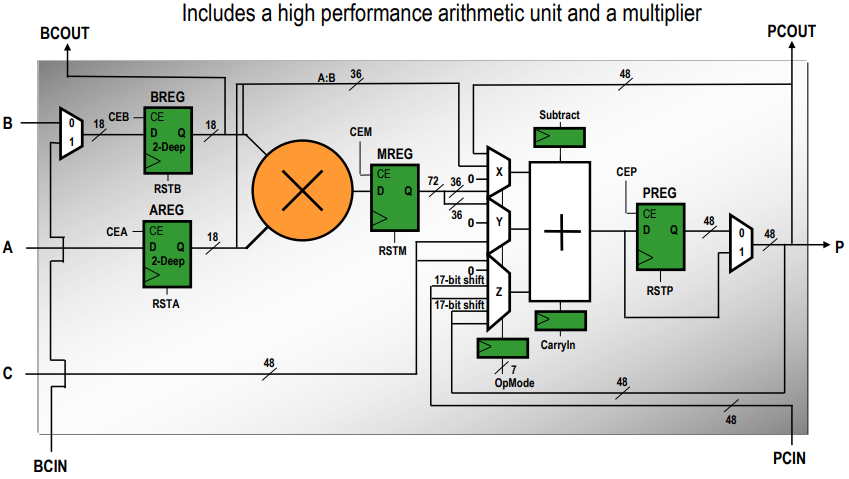
\includegraphics[width=\columnwidth]{img_2.png}
\end{figure}
\begin{itemize}
\item Plus de 40 opération possibles (7 bits OpMode)
\item Possibilité de changer l'opération à chaque coup d'horloge
\end{itemize}
\subsubsection{DSP48E}
Ajout de :
\begin{itemize}
\item ALU haute performance.
\item comparateur de pattern
\end{itemize}
\subsection{Utilisations}
\begin{itemize}
\item Charge de calcul importante
\item Calculs FIR rapides (parallélisation)
\item Calculs multi-canaux en parallèle
\item Architecture dédiée pour l'application (coût vs vitesse)
\item Intégration toute la logique dans une FPGA (réduction des coûts).
\end{itemize}

\subsection{Exemple de parcellisation : filtre FIR}
\begin{figure}[H]
\centering
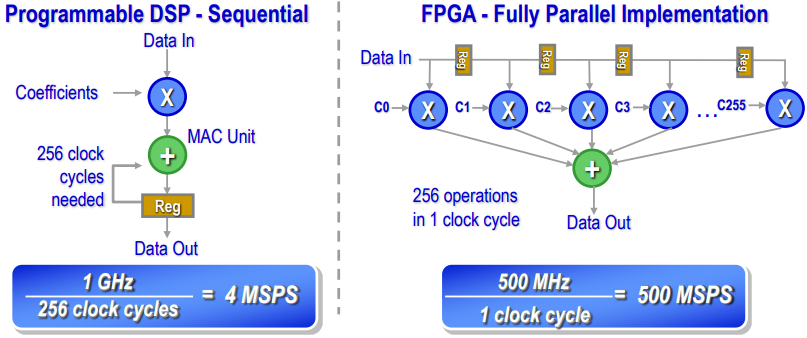
\includegraphics[width=\columnwidth]{img_3.png}
\end{figure}


\end{document}